\documentclass[a4paper]{article}
\usepackage[utf8]{inputenc}
\usepackage{amssymb}
\usepackage{amsmath}
\usepackage{amsthm} 
\usepackage{url}
\usepackage{xspace}
\usepackage{graphicx}
\usepackage[vlined]{algorithm2e} % lib for pseudo code
\usepackage{float}  % lib for pseudo code
\usepackage[T1]{fontenc}
\usepackage{pgfplots}
\usepackage{caption}
\usepackage{subcaption}
\usepackage{array}
\usepackage{mdframed}

\RestyleAlgo{boxruled}
\LinesNumbered


\newcolumntype{L}[1]{>{\raggedright\let\newline\\\arraybackslash\hspace{0pt}}m{#1}}

\graphicspath{ {Graphics/Images/} }

\usepackage{newunicodechar}
\newunicodechar{∙}{\cdotp}

\newcommand{\parahead}[1]{{\vspace*{6pt}\noindent\textbf{#1}\xspace\xspace\xspace\xspace}}

\newcommand{\heading}[1]{{\vspace{6pt}\noindent\sc{#1}}}

% Command for making <--> arrow with text above
\makeatletter
\newcommand\xleftrightarrow[2][]{%
  \ext@arrow 9999{\longleftrightarrowfill@}{#1}{#2}}
\newcommand\longleftrightarrowfill@{%
  \arrowfill@\leftarrow\relbar\rightarrow}
\makeatother

\newcommand{\vectorbound}{\ensuremath{\kappa}}
\newcommand{\secretbound}{\ensuremath{\nu}}
\newcommand{\E}{\ensuremath{\textnormal{E}}}
\newcommand{\Var}{\ensuremath{\textnormal{Var}}}
\newcommand{\U}[1]{\ensuremath{\mathcal{U}(#1)\xspace}}
\newcommand{\abs}[1]{\ensuremath{|#1|}\xspace}
\newcommand{\dotp}[2]{\ensuremath{\left\langle {#1},{#2}\right\rangle}\xspace}

\newcommand{\shortvec}[1]{\tilde{\mathbf{#1}}\xspace}
\renewcommand{\vec}[1]{\mathbf{#1}\xspace}
\newcommand{\cemph}[1]{\color{yellow9}{\bf #1}\xspace}
\newcommand{\chig}{\ensuremath{\chi_{\alpha,q}}}
\newcommand{\Z}{\ensuremath{\mathbb{Z}}\xspace}
\newcommand{\Zq}{\ensuremath{\Z_q}\xspace}
\newcommand{\ZqStar}{\ensuremath{\Z_q^*}\xspace}
\newcommand{\Zp}{\ensuremath{\mathbb{Z}_p}\xspace}
\newcommand{\Ldis}{L_{\mathbf{s},\chi}^{(n)}\xspace}
\newcommand{\sample}{\ensuremath{\leftarrow_{\$}}}
\renewcommand{\O}[1]{\ensuremath{{\mathcal{O}\left(#1\right)}}\xspace}
\newcommand{\round}[1]{\ensuremath{\left\lfloor{#1}\right\rceil}\xspace}
\newcommand{\Bdis}[1]{B_{\mathbf{s},\chi}(b,#1,p)\xspace}
\newcommand{\Bdissm}[1]{B_{small,\mathbf{s},\chi}(b,#1,p)\xspace}
\def\polyfactor{n\, \log_2^2 n}
\newcommand{\bigO}[1]{\ensuremath{\mathcal{O}\left(#1\right)}\xspace}
\newcommand{\svec}{\ensuremath{\mathbf{s}}\xspace} % command for pseudo code

\theoremstyle{plain}
\newtheorem{thm}{Theorem}[subsection]
\newtheorem{lemma}{Lemma}[subsection]
%\newmdtheoremenv[frametitlerule=true, frametitlebackgroundcolor=gray!20]{defi}

\mdfdefinestyle{defstyle}{frametitlerule=true, frametitlerulewidth=0px}
\mdtheorem[style=defstyle]{defi}{Definition}[subsection]

\mdtheorem[style=defstyle]{infobox}{}[subsection]

\title{Draft 1}
\author{Kasper and  Sune}
\date{February 2017}

\begin{document}

\maketitle

\begin{figure}[h]
    \centering
    \includegraphics[scale=0.1]{Ignacio.jpg}
    \caption{Ignacio Cascudo}
\end{figure}

\input{010_abstract.tex}

\section{Introduction}
In this master thesis we will study how to implement an  electronic voting scheme application which is based on some tools from cryptography where the most important tool is the Publicly Verifiable Secret Sharing (PVSS) protocol. The main paper for this protocol will be Berry Schoenmakers paper "A Simple Publicly Verifiable Secret Sharing Scheme and its Application to Electronic Voting" \cite{Schoenmakers1999}. \\\\
\noindent
Secret sharing is a tool which used in the PVSS protocol. Secret sharing is a way of distributing a secret among several servers. Secret sharing is where a dealer has a secret. The dealer shares pieces of the secret to each of the players. If there are a large number of players they will be able to reconstruct the secret. More technically the idea is to hide a secret inside of a polynomial so that given certain partial information of the polynomial we can recover the secret that was hidden in it.\\\\
\noindent
A Multiparty computation protocol (MPC) is a protocol which uses secret sharing and allows several parties to compute some function on some private inputs, in such a way that they learn the result but not the inputs from the other players. MPC is not using conventional methods, where some commonly trusted party, could gather sensitive information. The figure to the left is showing a judge who all participants trust to give their secret inputs. The trusted party can then compute the outcome of the process, for instance the sum of all inputs, and reveal the output. The right figure is equivalent MPC would work. Here there is no trusted party, but by using multiparty computation they can still achieve the same level of secrecy, but without having to trust someone.
 
\begin{center}
     \makebox[\textwidth]{\includegraphics[scale=0.35]{MPC.jpg}}
\end{center}

\noindent
This leads to a core observation namely that without a trusted party the ability to validate the input the MPC protocol relies on the participants honesty. 
The PVSS protocol used in this thesis proposes a solution to this problem. The idea is that not only can the participants verify their own shares, but that anybody can verify the correctness of the transmitted data.

\section{Motivation}
There are theoretical papers about how participants can communicate secure. For different reasons there are fewer papers which propose how to implement their theoretical results. This master thesis will try to combine a theoretical paper and how it actually can be implemented in a practical case. 

\section{Hypothesis}
Is it possible to create a secure practical usable electronic voting application based on the PVSS protocol. Before we can code an implementation it requires insight into the formal part of the cryptographically parts and then translate this into a proper implementation of the protocol. A goal for the implementation is to experiment with both small and large values and study how the application scales in time.




\section{Method}
To ensure structure the sections will be contructed based one or more of the following 3 methods.
\begin{enumerate}
    \item \textbf{General structure}  \\
    Informal description\\
    Definition\\
    Example\\
    Proof    
    \item \textbf{Zero-knowledge proof}
    \item \textbf{Pseudo code} 
\end{enumerate}

\parahead{General structure} The general rule will be that every section will start informal description of the subject. Here we will give a informal description of why this it is relevant to our rapport. After that a more formal description will come. Their will be parts where the formality will require a more in depth explanation. To avoid disruption we then put this formality last in the section.    


\parahead{Zero knowledge proof} In cryptography, a zero-knowledge proof or zero-knowledge protocol is a method by which one party (the prover) can prove to another party (the verifier) that a given statement is true, without conveying any information apart from the fact that the statement is indeed true. A zero-knowledge proof must satisfy following three properties:

%-----------------------------------------------zero knowledge
\begin{itemize}
\item  \textnormal{\textbf{(Completeness:)}} If the prover is honest it should pass or if the statement is true, the honest verifier (that is, one following the protocol properly) will be convinced of this fact by an honest prover.
\item    \textnormal{\textbf{(Soundness:)}} If the statement is false then it should fail with large probability or if the statement is false, no cheating prover can convince the honest verifier that it is true, except with some small probability..
\item   \textnormal{\textbf{(Zero-knowledge:)}} If the statement is true, no cheating verifier learns anything other than the fact that the statement is true. In other words, just knowing the statement (not the secret) is sufficient to imagine a scenario showing that the prover knows the secret. This is formalized by showing that every cheating verifier has some simulator that, given only the statement to be proved (and no access to the prover), can produce a transcript that "looks like" an interaction between the honest prover and the cheating verifier. In the PVSS protocol the receiver doesn't learn the \begin{math}x_i \end{math}.
\end{itemize}
%-----------------------------------------------zero knowledge

\parahead{Pseudo code} We will use pseudocode as an informal technique to outline the structure of our algorithms. This technique aims to describe a solution so that it is easy to read for humans.\\

\parahead{Indistinguishable}
The DLEQ proof involves this concept where the one cant distinguish between two values with the probability less than... Need reference..\\
\textcolor{red}{Sune: Måske droppes eller diskussion}





\section{Document Structure}
Here we present the content of the rapport. One section will contain the mathematical description of the protocol. The second section will be about the pratical part of the electronic voting application, where we will describe our implementation.


\input{044_Notation.tex}

\section{Modular arithmetic}
Modular arithmetic, is a simple way of performing arithmetic in a finite set of integers.

%**************************************Definition Modulo Operation Start
\begin{defi}[\textbf{Modulo Operation}]
Let \begin{math} a, r,m \in  \mathbb{Z}\end{math} (where \begin{math} \mathbb{Z}\end{math} is a set of all integers) and \begin{math} m > 0\end{math}. We write A 
\begin{center} \begin{math} a \equiv r \ mod \ m\end{math} \end{center}
if \begin{math}m \end{math} divides \begin{math} a - r \end{math}.\\
\begin{math}m \end{math} is called the modulus and \begin{math}r \end{math} is called the remainder.
\end{defi}
%**************************************Definition Modulo Operation End

\parahead{Computing the remainder} By example we can compute the remainder according to the definition. Given: \begin{math} a, m \in \mathbb{Z} \end{math} we compute the remainder by the following fomular:  \begin{math} a = qm +r \end{math}. The remainder is computed by how many times the quotient can be multiplied with the modulo. This example shows that the remainder is not unique. \\\\
\begin{math}42 = 4 * 9 +6 \implies r = 6 \end{math}, by definition \begin{math} (42-6) = 36 \end{math}, \begin{math} 9| 36 \end{math}\\
\begin{math}42 = 3 * 9 +15 \implies r = 15 \end{math}, by definition \begin{math} (42-15) = 27 \end{math}, \begin{math} 9| 27 \end{math}\\
\begin{math}42 = 5 * 9 +(-3) \implies r = -3 \end{math}, by definition \begin{math} (42-(-3)) = 45 \end{math}, \begin{math} 9| 45 \end{math}\\\\

\parahead{Equivalence classes} Above can also be written with the modulo operator. Here we show that all have different remainder but are in the same equivalence class modulo \textit{9}. This means that all members of a given equivalence class behave equivalently. Note also that one can compute with negative integers.

\begin{align*}
42 &= 6 \ mod \ 9 \\
42 &= 15 \ mod \ 9 \\
42 &= -3 \ mod \ 9 \\
\end{align*}
\parahead{Computing the inverse}
As we will see later, computing the inverse becomes an important part in this protocol for how to divide modulo an integer arithmetically. For this we have the Extended Euclidean algorithm which allows us to compute modular inverses given to positive integers. \\


\noindent
\parahead{Extended Euclidean algorithm} The first two lines (6-7) in the algorithm is the standard Euclidean Algorithm. It turns out that if we give the Extended Euclidean Algorithm $gcd(n,a)$, where $n$ is the modulo integer and $a$ is an integer, then the $t$ parameter will be the inverse of $a$. 

%**************************************Pseudocode Euclidean algorithm start
\begin{center}
\begin{algorithm}[H]
\caption{Extended Euclidean Algorithm (EEA)\label{alg}}

\SetKwRepeat{Do}{do}{while}

\KwIn{positive integers $r_0 $ and $r_1 $ with $r_0 $ > $r_1 $}
\KwOut{gcd($r_0 $, $r_1 $), as well as s and t such that gcd($r_0$, $r_1$) = $s * r_0+t * r_1 $.}

\textbf{Initialization:} \\
$
\begin{array}{ll}
    s_0 = 1   & t_0 = 0 \\
    s_1 = 0   & t_1 = 1 \\
      i = 1     &           \\
\end{array}                 
$

\Begin{
    \Do{$r_i \neq 0 $}{
    $i = i+1 $\\
    $r_i = r_{i-2} \ mod \ r_{i-1} $\\
    \begin{math} \mathbf{ q_{i-1} = ( r_{i-2}-r_{i} ) / r_{i-1} }  \end{math}\\
    $s_i = s_{i-2}-q_{i-1} * s_{i-1} $\\
    $t_i = t_{i-2}-q_{i-1} * t_{i-1} $
    }

\Return{ \\
    gcd($r_0 $, $r_1 $) = $r_{i-1} $\\
    s = $s_{i-1} $\\
    t = $t_{i-1} $
    }
}
\end{algorithm}
\end{center}


%**************************************Pseudocode Euclidean algorithm end

\parahead{Euclidean algorithm} The regular Euclidean algorithm works that given to integers $r_0 = 973$ and $r_1 = 301$, then the gcd is computed as 

\begin{center}
\begin{tabular}{|ll|lll| } 
\hline
$973$ & $= 3 \cdot 301 +70$& $gcd(973,301)$ & $= gcd(301,70)$ & \\ 
\hline
$301$ & $= 4 \cdot 70+21$ & $gcd(301,70)$ & $= gcd(70,21)$ &\\ 
\hline
$70$ & $= 3 \cdot 21+7$ & $gcd(70,21)$ & $= gcd(21,7)$ & \\ 
\hline
$21$ & $= 3 \cdot 7+0$ & $gcd(21,7)$ & $= gcd(7,0)$ & $= 7$ \\ 
\hline
\end{tabular}
\end{center}

\noindent
The core observation from this process is that we can reduce the problem of finding the gcd of two given numbers to that of the gcd of two smaller numbers.\\

\parahead{Example Extended Euclidean algorithm} On the left-hand side, we compute the standard Euclidean algorithm, i.e., we compute new remainders $r_2$, $r_3$, ... Also, we have to compute the integer quotient $q_{i-1}$ in every iteration. On the right-hand side we compute the coefficients $s_i$ and $t_i$ such that $r_i = s_i r_0 + t_i r_1$. 
\begin{center}
\begin{tabular}{|l|l|p{5cm}| } 
\hline
$i$ & $r_{i-2} = q_{i-1} \cdot r_{i-1}+r_i$ & $r_i = [s_i]r_0 +[t_i]r_1$ \\ 
\hline
$2$ & $973 = 3 \cdot 301 +70$& $r_2=70= [1] 973 + [-3]301$ \\ 
\hline
$3$ & $301 = 4 \cdot 70+21$ & $r_3= 21= 301-4 \cdot 70$ \newline $ r_3 = 301 -4(973-3 \cdot 301)$ \newline $r_3 = [-4]973 + [13]301$\\
\hline
$4$ & $70 = 3 \cdot 21+7$ & $r_4= 70 - 3 \cdot 21$ \newline $r_4=(973-3 \cdot 301) -3(4 \cdot 973 + 13 \cdot 301)$ \newline $r_4=[13]973+[42] 301$  \\ 
\hline
\end{tabular}
\end{center}

\noindent
To understand the how the EEA works we observe that the righthand side is always constructed with the help of the previous linear combinations. We will now derive recursive formulae for computing $s_i$ and $r_i$ in every iteration. Assume we are in iteration with index i. 

\begin{infobox}[The two previous iterations we computed the values]
$r_{i - 2} = [s_{i-2}]r_0 +[t_{i-2}]r_1$\\
$r_{i-1} = [s_{i-1}]r_0 +[t_{i-1}]r_1$
\end{infobox}

\noindent
In the current iteration i we first compute the quotient $q_{i-1}$ and the new remainder $r_i$ from $r_{i-1}$ and $r_{i-2}$:

\begin{infobox}[Current iteration $i$]
$r_{i-2} = q_{i-1} \cdot r_{i-1}+r_i$.\\
This equation can be rewritten as:\\
$r_i = r_{i-2}-q_{i-1} \cdot r_{i-1}$.
\end{infobox}


\noindent
The goal is to represent the new remainder $r_i$ as a linear combination of $r_0$ and $r_1$ as $r_i = [s_i]r_0 +[t_i]r_1$. The core step for achieving this is by substitute $r_{i-2}$ and $r_{i-1}$ by the following.

\noindent
\begin{infobox}[Substitute $r_{i-2}$ and $r_{i-1}$]
$r_i = (s_{i-2}r_0+t_{i-2}r_1)-q_{i-1}(s_{i-1}r_0+t_{i-1}r_1)$\\
If we rearrange the terms we obtain the desired result:\\
$r_i = [s_{i-2}-q_{i-1}s_{i-1}]r_0 +[t_{i-2}-q_{i-1}t_{i-1}]r_1$\\
$r_i = [s_i]r_0 +[t_i]r_1$
\end{infobox}

\input{047_Group_Theory.tex}

\section{Mathematical tools}
The following section will be about the cryptographic assumptions which are used in the PVSS protocol. We will also describe some techniques which will be used in practical part of coding the protocol.

%------------------------------------------------------------------------------------
\subsection{One-way function and The Discrete logarithm problem} % and One way functions
%------------------------------------------------------------------------------------

\parahead{One-way function} One-way functions are easy to compute but it is very difficult to compute their inverse functions. Thus, having data $x$ it is easy to calculate $f(x)$ but,  
knowing only the result of $f(x)$ it is hard to calculate the value of $x$. We say a function $f(x)$ is easy to compute if this can be done in polynomial running time. 
In order to be useful in practical crypto schemes, the computation of $f(x)$ should be fast enough that it does not lead to unacceptably slow execution times in an application. The inverse
computation of $f(x)$ should be so computationally intensive that it is not feasible to evaluate it in any reasonable time period. We define a One-way function as \\

\begin{defi}[One-way function]
A function $f()$ is a one-way function if:      \\
1. $y = f (x)$ is computationally easy           \\
2. $x = f^{-1}(y)$ is computationally infeasible    
\end{defi}

\noindent
An example of a one-way function is $n = pq$ where $p$ and $q$ are primes, it is easy to compute $n$ given $p$ and $q$ but hard to find $p$ and $q$ given only $n$. 
Inverting this function requires finding the factors of $n$.
An other example of a one-way function is Discrete logarithm. \\


\parahead{Discrete logarithm (DL)} A discrete logarithm is a integer $a$ exponent that solves $g^a=c$, where $g$ is a generator and $c$ is a element of a cyclic group. Given $a$ its easy to compute, but given only $g$ and $c$ its very hard to find $a$. We define discrete logarithm as \\

\begin{defi}[Discrete logarithm (DL) problem]
Given a group $G$, generator $g$ and $c \in G$, find integer $a$, such that $g^a = c$
\end{defi}

\noindent
An example of the DL problem could be the following. Given a group $G = \Z_47^*$, an generator $g=5$, and an element $c = 41$ find a integer $a$ to solve: 

\begin{center}
$
\begin{array}{l}
     5^a \stackrel{?}{=} 41 \ mod \ 47 \\
     \\
     \text{To solve this DL problem we need to find} \\
     a = 15 \ as \ 5^{15} = 41 \ mod \ 47
\end{array}
$
\end{center}

\noindent
To solve this DL problem we could just tried all possible solution of \\
$ \{g^0, g^1, g^2,...,g^{46}\} \ mod \ 47$ until we find the correct answer. However it is easy to see that given a large enough group this would be ineffective, actually the DL problem is believed to be notoriously hard, for instance in $\Z_p^*$ for large prime $p$. \\

\noindent
We use the DL problem in the following

% Comment out since Kl dont know if we need this. 
\iffalse
    \begin{defi}[Computational Diffie-Hellman (CDH) problem]
    \begin{math}g\in\Z_p, \ g\neq1 \end{math}\\
    Given \begin{math}(g,g^a,g^b)\end{math} find(compute)  \begin{math}(g^{a*b})\end{math} is hard problem.\\
    Definition: Need a reference?? \\
    \textcolor{red}{Kasper}
    \end{defi}
\fi

\parahead{Diffie-Hellman problem (DHP)}
One of the best known application of the DL problem is in the Diffie-Hellman problem an in particular in the Diffie-Hellman key exchange. Though the Diffie-Hellman key exchange is not used in the PVSS protocol we will use it to illustrate the DHP.


\begin{figure}[H]
    \centering        
    
    $
    \begin{array}{l}
    \hline                      \
    \textbf{Diffie-Hellman Key Exchange}      \\
    \hline                      \\
    \text{Public: a group G and a generator g}      \\
    \\
	\begin{array}{L{1.1cm}lcl}
        & \text{\textsf{Alice}} & \text{\textsf{Eve}}_{Adversery} & \text{\textsf{Bob}} \\
        \hline
        Step \ 1    &           \begin{array}{l}
                                   Chose: \ a \in_R G        \\ 
                                   Compute: \ A = g^a         
                                \end{array}     & \xrightarrow{\hspace{3em} A \hspace{3em}}  & \\
        Step \ 2    &                           & \xleftarrow{\hspace{3em} B \hspace{3em}}       &                                                    \begin{array}{l}
                                                            Chose: \ b \in_R G \\
                                                            Compute: \ B = g^b
                                                        \end{array} \\
                    \\
        Step \ 3    &   \begin{array}{ll} 
                            C &= (B)^a      \\
                              &= (g^b)^a    \\
                              &= g^{ab}
                        \end{array}   &     \xleftrightarrow{\hspace{0.5em}encrypt_C(message)\hspace{0.5em}} & \begin{array}{ll} 
                            C &= (A)^b      \\
                              &= (g^a)^b    \\
                              &= g^{ab}     
                        \end{array}     \\                                                 
        \hline
    \end{array}
    \end{array}
    $    
    \caption{Diffie-Hellman Key Exchange}
	\label{fig:Diffie_Hellman_KeyExchange}
\end{figure}

\noindent
As shown in step 1 Alice is independently from Bob choosing an random element from the group G and using this to create a DL problem A which is sent to Bob. In step 2 Bob is doing the procedure as Alice and sends a DL problem B to Bob. In step 3 they both independently from each other using the received DL problems to create a key C. Both Alice and Bob will compute the same value C which can be used as a key in a cryptographic scheme. \\

\noindent
If we look at the exchange from Eve's point of view, we can see that Eve knows the public elements G and g aswell as A and B from step 1 and 2. If Eve can compute $C = g^{ab}$ then Eve would be able to decrypt any message sent between Alice and Bob. We define this problem as. \\

\begin{defi}[Computational Diffie-Hellman (CDH) problem]
Given a group $G$, generator $g$ and $A = g^a$, $B = g^b$, where $a,b$ is are randomly independently chosen from $\Zp$, compute $C=g^{ab}$ 
\end{defi}

\noindent
If Eve knows an efficient algorithm to solve the DL problem, then Eve would also be able to solve the CDH problem. Finding $a$ from $A = g^a$ or $b$ from $B = g^b$ then Eve can easily compute $C$ the same way that Alice and Bob was able to. which leads us to  

\begin{lemma}
The CDH problem is no harder then the DL problem
\end{lemma}

\noindent
It is not known if the opposite direction is true in general, but in some groups, the problems are equivalent. The CDH problem have another property namely if given a group element and the claim that this solves a CDH instance, then is not easy to verify that the solution is correct unless  we can solve the DL problem.  




We would need to decide if, given $g^a, g^b, g^c$, it holds that $c = ab \ mod \ p$. This leads us to the final related problem \\

\parahead{Decisional Diffie-Hellman (DDH) problem} The idea with DDH is that given a instance of the CDH problem plus an group element which is either a correct CDH solution, or is a random element. Then we are to guess which case we are in. We define the DDH problem as \\

\iffalse
    \begin{defi}[Decisional Diffie-Hellman (DDH) problem]
    \begin{math}g\in\Z_p, \ g\neq1 \end{math}\\ 
    Given \begin{math}(g,g^a,g^b,g^c)\end{math} decide if  \begin{math}(a*b=c)\end{math} is hard problem.\\
    Definition: Need a reference??
    \end{defi}
\fi 

\begin{defi}[Decisional Diffie-Hellman (DDH) problem] 
    Given a group $G$, a generator $g$ and $A = g^a$, $B = g^b$ and $C = g^c$, where $a$ and $b$ are randomly and independently chosen from $\Z_p$ and where $c$ is chosen either as $c = ab$ or uniformly random from $\Zp$. Now guess which of the two cases we are in.   
\end{defi}

The DDH problem essentially comes down to deciding if $\delta = CDH(G,g,\beta,\gamma)$. This can however also happen when $c$ is randomly chosen but only with by a very small probability $1 / p$. 
\noindent
We use $DDH(G,g,\beta,\gamma) \in \{0,1\}$ to denote the solution, where $DDH(G,g,\beta,\gamma) = 1$ if $CDH(G,g,\beta,\gamma) = \delta$ and $DDH(G,g,\beta,\gamma) = 0$ if $CDH(G,g,\beta,\gamma) \neq \delta$.

We can see that if we can solve the CDH problem then we can solve the DDH problem simply by computing $g^{ab}$ and comparing it with $g^c$. So we have 

\begin{lemma}
The DDH problem is no harder then CDH problem
\end{lemma}


\parahead{In the PVSS protocol}  
\textcolor{red}{Needs some more filling :)}

The security of the PVSS protocol can be reduced down to the hardness of the DL problem. Which means that if there can be found a efficient algorithm to solve the DL problem with large expoents then the entire PVSS protocol is insecure. In the next subsection we will look at known algorithms for solving the DL problem. 


%------------------------------------------------------------------------------------
\subsection{Known algorithms for solving the Discrete Logarithm Problem}
%------------------------------------------------------------------------------------
\begin{enumerate}
    \item \textbf{Brute-force / Exhausted search} \\
    Running time: \bigO{n}
    
    \item \textbf{Square-root attacks} \\
    The Square-root attacks works in any group. \\
    Running time: \bigO{\sqrt{n}}
    
    \begin{enumerate}
        \item Baby-steps Giant-steps algorithm
        \item Pollard's rho algorithm
    \end{enumerate}
    \item \textbf{Index-Calculus attacks} \\
    Index-Calculus attacks are the best known attack against DLP, but it only
    works in certain groups, in particularly $\Z_p^* $ and $ GF(2^m)^* $. \\
    
    This means in practice that $p$ needs to between $ 2^{1024} $ to $ 2^{2048} $
\end{enumerate}

\noindent
\parahead{Baby-steps Giant-steps algorithm} Kasper Lemming er sej!!

\textcolor{red}{Kasper is working on this}



%------------------------------------------------------------------------------------
\subsection{Hash function}
%------------------------------------------------------------------------------------
Hash functions is a function that takes a message of arbitrary size and outputs a digest hash value of a fixed size. The hash functions used in this project is hash function, which means that they are considered as one-way function. we define cryptographic hash function, denote just as hash functions onward, as.

\begin{defi}[Hash function]
\begin{enumerate}
    \item Takes a message of arbitrary size and outputs a value of fixed size
    \item Is deterministic so the same message always results in the same hash
    \item Is quick to compute the hash value for any given message
    \item Is collision resistant, mean it is infeasible to find two inputs $x$ and $x'$ such that $H(x) = H(x')$, and $x \neq x'$
    \item A small change to a message should change the hash value so extensively that the new hash value appears uncorrelated with the old hash value
\end{enumerate}
\end{defi}

A function hash function: $\{0,1\}^{\leq L} \rightarrow \{0,1\}^\ell$ is called collision resistant if it is hard to find $x \in \{0,1\}^{\leq L}$ and $x' \in \{0,1\}^{\leq L}$ such that $x \neq x'$ and $H(x)=H(x')$ - the value $(x,x')$ is called a collision. Here $\{0,1\}^{\leq L}$ denotes the set of bitstrings of length at most $L$. If $L \geq \ell$, then of course collisions exist, so they can be found given enough time, which is fine as we only ask that they are computationally hard to find.  

%------------------------------------------------------------------------------------
\subsection{Homomorphic Secret Sharing}
%------------------------------------------------------------------------------------
A homomorphism is a transformation from one algebraic structure into another of the same type so that the structure is preserved. Importantly, this means that for every kind of manipulation of the original data, there is a corresponding manipulation of the transformed data.\\

\noindent 
A homomorphic encryption scheme is a crypto system that allows computations to be performed on data without decrypting it. It is an encrypting scheme which allows computations to be carried out on ciphertext, thus generating an encrypted result which, when decrypted, matches the result of operations performed on the plaintext.\\

\noindent
\parahead{Homomorphic Secret Sharing} is a type of secret sharing algorithm in which the secret is encrypted via homomorphic encryption. In the PVSS scheme we use this property that one can sum the shares which are equal to the sum of the secrets.

\begin{defi}[Homomorphic Secret Sharing]
\begin{math}s\rightarrow (s_i,...,s_n)\end{math}\\
\begin{math}u\rightarrow (u_i,...,u_n) \end{math}\\
\begin{math}s+u\rightarrow (s_i+u_i,...,s_n+u_n) \end{math}\\
\textcolor{red}{Ignacio: We need a formal definition. In "Introduction to Modern Cryptography" there are explanation on Homomorphic encryption page.499. It is correct understood that we use the property of Homomorphic Secret Sharing in section 12.3 }
\end{defi}


%------------------------------------------------------------------------------------
\subsection{Fiat Sharmir}
%------------------------------------------------------------------------------------
The Fiat–Shamir heuristic is a technique in cryptography for taking an interactive proof of knowledge into a non interactive proof (signature scheme). This way, some fact (for example, knowledge of a certain number secret to the public) can be proven without revealing underlying information. This means that transforming a interactive proof into a non-interactive proof. Instead of the verifier creates a challenge the prover creates a challenge, on some previous data, based on a hash function.

\begin{figure}[H]
    \centering        
    
    $
    \begin{array}{l}
    \hline                      \
    \textbf{Fiat Sharmir}      \\
    \hline                      \\
    \text{Public: identification schemes} \ Gen_{id}, P_1, P_2, V       \\
    \text{The Signer: Private key} \ sk \text{, public key} \ pk \text{, message} \ m \in \{1,0\}  \\
    \\
	\begin{array}{L{1.1cm}lcl}
        & \text{\textsf{Signer}}_{sk,pk, m} & & \text{\textsf{Verifier}} \\
        \hline
        Step \ 1    &           \begin{array}{l}
                                    (I,st) \leftarrow P_1(sk)             \\ 
                                    r := H(I,m)      \\ 
                                    s := P_2(sk,st,r)    
                                \end{array}     &                                   & \\
                    &                           &                                   & \\
        Step \ 2    &                           &       \xrightarrow{\hspace{1em} r, \ s, \ pk \hspace{1em}} & \begin{array}{l}
                                                            Compute: \\ 
                                                            I := V(pk,r,s) \\ \\
                                                            Outputs: \\ 
                                                            1 \ \text{if and only if} \ H(I,m) \stackrel{?}{=} r \\
                                                        \end{array} \\
        \hline
    \end{array}
    \end{array}
    $    
    \caption{Fiat Sharmir}
	\label{fig:Fiat__Sharmir}
\end{figure}

\begin{defi}[Fiat Sharmir]
\textcolor{red}{Ignacio: We need a formal definition}
\textcolor{red}{Ignacio: explanation of identification schemes to signatures 453 - 456 (Introduction to Modern Cryptography) }
\end{defi}


\noindent






\section{Shamir Secret Sharing}
\parahead{Secret sharing} is a way of distributing a secret among several servers. Adi Shamir, one of the most important cryptographers of our time came up with the idea of using polynomials for this protocol. The idea is to hide a secret inside of a polynomial so that given certain partial information of the polynomial we can recover the secret that was hidden in it.\\ \\
Basically it is about hiding information in a polynomial \begin{math}p\end{math}. For example, a voter chooses a random polynomial of the degree 1, which is a line. The secret is the evaluation of the polynomial in \begin{math}p(0)\end{math}. Each server receive a share, the evaluation of  \begin{math}p\end{math} in some other point. Like as server  1 receives  \begin{math}p(1)\end{math}, server 2 receives \begin{math}p(2)\end{math} and etc. To construct the line we need at most two point. One can see that if we don’t have at least 2 points then the line can be constructed in many ways, which is the same as saying we don’t know the evaluation of \begin{math}p(0)\end{math}.\\ \\
In the general case, the polynomial is chosen to be of degree \textit{t}. The scheme requires we need 
 \begin{math}t+1\end{math} points to reconstruct the secret. This means that if we have \textit{t}-servers they would not be able to obtain anything about the secret. 

\parahead{Passive corruption} is that a server (semihonest) gets access to information which the server is not entitled to, e.g. if a voter ask another voter about his information and tries to compare the information and get some more information in that way. By using secret sharing we can prevent passive corruption, because the scheme guaranties that if \textit{t}-servers are corrupted then they will not be able to gain anything.


\parahead{Active corruption} happens when the voters (malicious) try to send values that they are not supposed to send - so the voters deviate from the protocol. \\
\textcolor{red}{Ignacio: according to "Introduction to Modern Cryptography" page 503 the verifiable secret sharing scheme prevent two separate concerns on active corruption. Does this also hold for the PVSS scheme -can you please elaborate that. }


\subsection{Lagrange interpolation}
The idea is that we know some evaluations points. With Lagrange interpolation, we have a formula, with which we can reconstruct the polynomial.
The general formula, Lagrange interpolation, looks like:



\begin{defi}[Lagrange polynomial interpolation]
\begin{math}p(x)=\sum\limits_{i \in C} p(i)\lambda_i(x)\end{math}, where $\lambda_i(x)$ is defined by \begin{math} \lambda_i(x)=\prod\limits_{j\in C,j\neq i}  \frac{x-j}{i-j} \end{math}
\end{defi}



\noindent
In secret sharing scheme each server get some shares ("points") and if there are enough servers then the servers can reconstruct the secret by reconstructing the polynomial. By example we will show how the formula works.  We have a polynomial \textit{p}, where we know the evaluation of some points.

\begin{figure}[H]
    \centering
    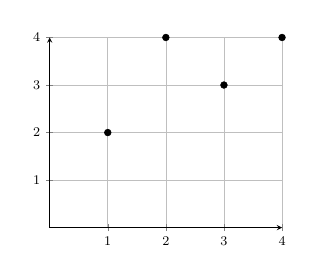
\begin{tikzpicture}[scale=0.6]
    \begin{axis}[
            grid = major,
            xmin=0, xmax=4,
            ymin=0, ymax=4,
            axis lines=center,
            axis on top=true,
            small,
            domain=0:4,
        ]
        \addplot[only marks, color = black, mark = *]
        table[meta=label] {
            x       y       label
            1       2       a
            2       4       a
            3       3       a
            4       4       a
        };
    \end{axis}
    \end{tikzpicture} 
    \caption{polynomial p}
\end{figure}

\noindent
Instead of solving the polynomial, we will start to divide the problem into smaller pieces and solve them one by one. We create a polynomial,\begin{math} \lambda_1, \lambda_2, \lambda_3\end{math} and \begin{math}\lambda_4\end{math}, one for each point from polynomial \textit{p}. These polynomial takes value 1 in one point and 0 in the other points. For example \begin{math} \lambda_1\end{math} takes 1 in 1 and 0 in 2,3 and 4.

\begin{figure}[H]
    \centering
    \captionsetup[subfigure]{labelformat=empty}
    \begin{subfigure}[b]{0.3\textwidth}
        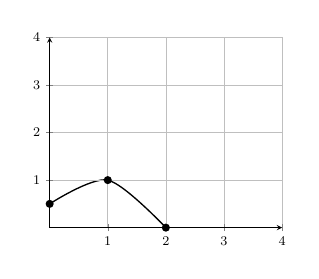
\begin{tikzpicture}[scale=0.6]
        \begin{axis}[
                grid = major,
                xmin=0, xmax=4,
                ymin=0, ymax=4,
                axis lines=center,
                axis on top=true,
                small,
            ]
            \addplot[smooth, thick, color = black, mark = *]
            table[meta=label] {
                x       y       label
                0       0.5     a
                1       1       a
                2       0       a
            };
        \end{axis}
        \end{tikzpicture} 
        \caption{approximately $\lambda_1$}
    \end{subfigure}
    \qquad % <----------------- SPACE BETWEEN PICTURES
    \qquad % <----------------- SPACE BETWEEN PICTURES
    \qquad % <----------------- SPACE BETWEEN PICTURES
    \qquad % <----------------- SPACE BETWEEN PICTURES
    \begin{subfigure}[b]{0.3\textwidth}
        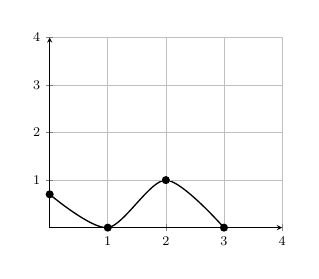
\begin{tikzpicture}[scale=0.6]
        \begin{axis}[
                grid = major,
                xmin=0, xmax=4,
                ymin=0, ymax=4,
                axis lines=center,
                axis on top=true,
                small,
            ]
            \addplot[smooth, thick, color = black, mark = *]
            table[meta=label] {
                x       y       label
                0       0.7     a
                1       0       a
                2       1       a
                3       0       a
            };
        \end{axis}
        \end{tikzpicture} 
        \caption{approximately $\lambda_2$}
    \end{subfigure}
\end{figure}

\noindent
Note that the evaluation in 0 will depend on the secret. For the sake of the drawings it is just an approximately of the point.

\begin{figure}[H]
    \centering
    \captionsetup[subfigure]{labelformat=empty}
    \begin{subfigure}[b]{0.3\textwidth}
        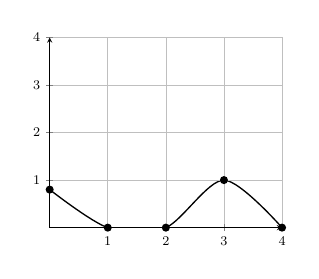
\begin{tikzpicture}[scale=0.6]
        \begin{axis}[
                grid = major,
                xmin=0, xmax=4,
                ymin=0, ymax=4,
                axis lines=center,
                axis on top=true,
                small,
            ]
            \addplot[smooth, thick, color = black, mark = *]
            table[meta=label] {
                x       y       label
                0       0.8     a
                1       0       a
                2       0       a
                3       1       a
                4       0       a
            };
        \end{axis}
        \end{tikzpicture} 
        \caption{approximately $\lambda_3$}
    \end{subfigure}
    \qquad % <----------------- SPACE BETWEEN PICTURES
    \qquad % <----------------- SPACE BETWEEN PICTURES
    \qquad % <----------------- SPACE BETWEEN PICTURES
    \qquad % <----------------- SPACE BETWEEN PICTURES
    \begin{subfigure}[b]{0.3\textwidth}
        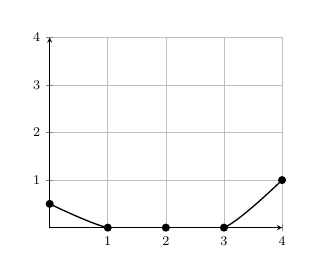
\begin{tikzpicture}[scale=0.6]
        \begin{axis}[
                grid = major,
                xmin=0, xmax=4,
                ymin=0, ymax=4,
                axis lines=center,
                axis on top=true,
                small,
            ]
            \addplot[smooth, thick, color = black, mark = *]
            table[meta=label] {
                x       y       label
                0       0.5     a
                1       0       a
                2       0       a
                3       0       a
                4       1       a
            };           
        \end{axis}
        \end{tikzpicture} 
        \caption{approximately $\lambda_4$}
    \end{subfigure}
\end{figure}

\noindent
To construct the polynomial \begin{math}p\end{math} is to take each polynomials and multiply the corresponding coefficient from \begin{math}p\end{math} and then sum the polynomials together \begin{math}2∙\lambda_1+4∙\lambda_2+3∙\lambda_3+4∙\lambda_4 \end{math}. We started with the \begin{math}\lambda\end{math} polynomial and we ended with four polynomials, which takes value 2,4,3,4 and 0 in the other points. From the sum we see that the value in the first point 2+0+0+0. It is clear this will work in the other points. 

\begin{figure}[H]
    \centering
    \captionsetup[subfigure]{labelformat=empty}
    \begin{subfigure}[b]{0.3\textwidth}
        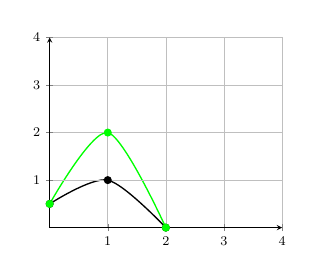
\begin{tikzpicture}[scale=0.6]
        \begin{axis}[
                grid = major,
                xmin=0, xmax=4,
                ymin=0, ymax=4,
                axis lines=center,
                axis on top=true,
                small,
            ]
            \addplot[smooth, thick, color = black, mark = *]
            table[meta=label] {
                x       y       label
                0       0.5     a
                1       1       a
                2       0       a
            };
            \addplot[smooth, thick, color = green, mark = *]
            table[meta=label] {
                x       y       label
                0       0.5     a
                1       2       a
                2       0       a
            };             
        \end{axis}
        \end{tikzpicture} 
        \caption{approximately $\lambda_1$}
    \end{subfigure}
    \qquad % <----------------- SPACE BETWEEN PICTURES
    \qquad % <----------------- SPACE BETWEEN PICTURES
    \qquad % <----------------- SPACE BETWEEN PICTURES
    \qquad % <----------------- SPACE BETWEEN PICTURES
    \begin{subfigure}[b]{0.3\textwidth}
        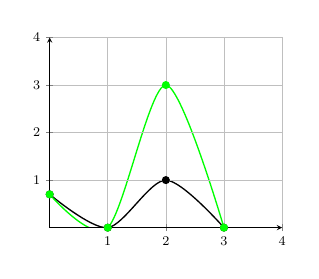
\begin{tikzpicture}[scale=0.6]
        \begin{axis}[
                grid = major,
                xmin=0, xmax=4,
                ymin=0, ymax=4,
                axis lines=center,
                axis on top=true,
                small,
            ]
            \addplot[smooth, thick, color = black, mark = *]
            table[meta=label] {
                x       y       label
                0       0.7     a
                1       0       a
                2       1       a
                3       0       a
            };
            \addplot[smooth, thick, color = green, mark = *]
            table[meta=label] {
                x       y       label
                0       0.7     a
                1       0       a
                2       3       a
                3       0       a
            };             
        \end{axis}
        \end{tikzpicture} 
        \caption{approximately $\lambda_2$}
    \end{subfigure}
\end{figure}

\begin{figure}[H]
    \centering
    \captionsetup[subfigure]{labelformat=empty}
    \begin{subfigure}[b]{0.3\textwidth}
        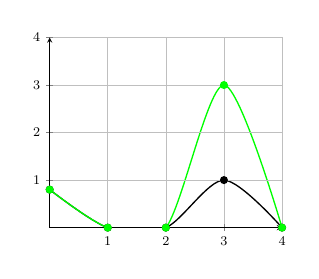
\begin{tikzpicture}[scale=0.6]
        \begin{axis}[
                grid = major,
                xmin=0, xmax=4,
                ymin=0, ymax=4,
                axis lines=center,
                axis on top=true,
                small,
            ]
            \addplot[smooth, thick, color = black, mark = *]
            table[meta=label] {
                x       y       label
                0       0.8     a
                1       0       a
                2       0       a
                3       1       a
                4       0       a
            };
            \addplot[smooth, thick, color = green, mark = *]
            table[meta=label] {
                x       y       label
                0       0.8     a
                1       0       a
                2       0       a
                3       3       a
                4       0       a
            };            
        \end{axis}
        \end{tikzpicture} 
        \caption{approximately $\lambda_3$}
    \end{subfigure}
    \qquad % <----------------- SPACE BETWEEN PICTURES
    \qquad % <----------------- SPACE BETWEEN PICTURES
    \qquad % <----------------- SPACE BETWEEN PICTURES
    \qquad % <----------------- SPACE BETWEEN PICTURES
    \begin{subfigure}[b]{0.3\textwidth}
        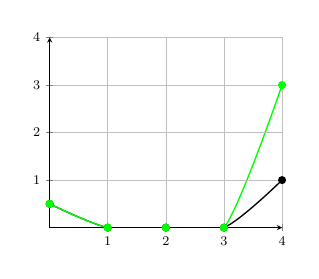
\begin{tikzpicture}[scale=0.6]
        \begin{axis}[
                grid = major,
                xmin=0, xmax=4,
                ymin=0, ymax=4,
                axis lines=center,
                axis on top=true,
                small,
            ]
            \addplot[smooth, thick, color = black, mark = *]
            table[meta=label] {
                x       y       label
                0       0.5     a
                1       0       a
                2       0       a
                3       0       a
                4       1       a
            };
            \addplot[smooth, thick, color = green, mark = *]
            table[meta=label] {
                x       y       label
                0       0.5     a
                1       0       a
                2       0       a
                3       0       a
                4       3       a
            };               
        \end{axis}
        \end{tikzpicture} 
        \caption{approximately $\lambda_4$}
    \end{subfigure}
\end{figure}


\noindent
We will now construct one of the \begin{math}\lambda\end{math}-polynomials by example, by showing it from \begin{math}\lambda_1\end{math} polynomial. 
We have the following points \begin{math}\lambda_1(1)=1, \lambda_1(2)=0, \lambda_1(3)=0 \end{math} and \begin{math} \lambda_1 (4)=0\end{math}. We take the polynomial \begin{math} (x-2)(x-3)(x-4)\end{math}, and we see that if we get correct evaluation in \begin{math}\lambda_1 (2)=0, \lambda_1 (3)=0\end{math} or \begin{math} \lambda_1 (4)=0\end{math}. To get correct evaluation in  \begin{math} \lambda_1 (1)=1\end{math} we divide by \begin{math}-6\end{math} because we see that \begin{math}(1-2)(1-3)(1-4)=-6\end{math} and then we end up with a polynomial \begin{math}\frac{(x-2)(x-3)(x-4)}{(-6)}\end{math} .  The polynomial still satisfies the conditions because when we divide zero with "something" we get zero.  The formula for constructing \begin{math}\lambda_1\end{math} 

\begin{center}
\begin{math} \lambda_1(x)=\prod\limits_{j\in C,j\neq1} \frac{x-j}{1-j} = \frac{x-2}{1-2}*\frac{x-3}{1-3}*\frac{x-4}{1-4}=\frac{(x-2)(x-3)(x-4)}{-6} \end{math}\\
\end{center}

\noindent
\begin{math} \lambda_1\end{math} gives 1 in point 1 and 0 in the other points. What this mean is that in \begin{math} \lambda_1(1)=1\end{math} and all other points  \begin{math}j (2,3,4)\end{math} we have \begin{math} \lambda_1 (j)=0\end{math}. We can construct \begin{math}\lambda_1, \lambda_2, \lambda_3\end{math} and  \begin{math}\lambda_4\end{math} in the same way.

\begin{center}
\begin{math} \lambda_2(x)=\prod\limits_{j\in C,j\neq2} \frac{x-j}{2-j} = \frac{x-1}{2-1}*\frac{x-3}{2-3}*\frac{x-4}{2-4}=\frac{(x-1)(x-3)(x-4)}{-2} \end{math}\\ \begin{math} \lambda_3(x)=\prod\limits_{j\in C,j\neq3} \frac{x-j}{3-j} = \frac{x-1}{3-1}*\frac{x-3}{3-2}*\frac{x-4}{3-4}=\frac{(x-1)(x-2)(x-4)}{-2} \end{math}\\ \begin{math} \lambda_4(x)=\prod\limits_{j\in C,j\neq4} \frac{x-j}{4-j} = \frac{x-1}{4-1}*\frac{x-3}{4-2}*\frac{x-3}{4-3}=\frac{(x-1)(x-2)(x-3)}{-6} \end{math}\\ \end{center}

\noindent
With the knowledge of the evaluation of \begin{math}p(1), p(2), p(3)\end{math} and  \begin{math}p(4)\end{math} we construct the formula for polynomial evaluation in \begin{math}p(0)\end{math}:


\noindent
\begin{infobox}[Applying Lagrange polynomial interpolation for polynomial evaluation in $0$]
We use the formula \begin{math}p(x)=\sum\limits_{i \in C} p(i)\lambda_i(x)\end{math} and we get the evaluation on some polynomial in $0$
\begin{center}
\begin{math}p(0)=p(1)∙\lambda_1+p(2)∙\lambda_2+p(3)∙\lambda_3+p(4)∙\lambda_4=2∙\lambda_1+4∙\lambda_2+3∙\lambda_3+4∙\lambda_4 \end{math}
\end{center}
\label{info:Applying_Lagrange_polynomial_interpolation}
\end{infobox}



\noindent
The idea of constructing the smaller polynomials is that we can reuse them for constructing other polynomials. From the smaller pieces and the evaluation points we can construct the polynomial from Lagrange interpolation. From the secret sharing scheme we know the degree of the polynomial is bounded. Because the voter will share its secret by choosing a random polynomial of the degree at most \textit{t}. That’s a guaranty we have from the scheme. If the degree of $p(x)$ is at most \textit{t} meaning $p(x)\leq t$. Then we need $t+1$ point to reconstruct the $p(x)$. If the degree 1 (line) then we need two points. The parable is where the degree is 2, here we need 3 points to construct
the polynomial.

\begin{figure}[H]
    \centering
    \captionsetup[subfigure]{labelformat=empty}
    \begin{subfigure}[b]{0.3\textwidth}
        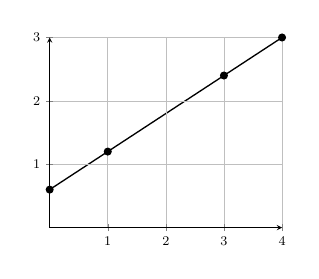
\begin{tikzpicture}[scale=0.6]
        \begin{axis}[
                grid = major,
                xmin=0, xmax=4,
                ymin=0, ymax=3,
                axis lines=center,
                axis on top=true,
                small,
            ]
            \addplot[smooth, thick, color = black, mark = *]
            table[meta=label] {
                x       y       label
                0       0.6     a
                1       1.2     a
                3       2.4     a
                4       3       a
            };
        \end{axis}
        \end{tikzpicture} 
        \caption{polynomial of degree 1}
    \end{subfigure}
    \qquad % <----------------- SPACE BETWEEN PICTURES
    \qquad % <----------------- SPACE BETWEEN PICTURES
    \qquad % <----------------- SPACE BETWEEN PICTURES
    \qquad % <----------------- SPACE BETWEEN PICTURES
    \begin{subfigure}[b]{0.3\textwidth}
        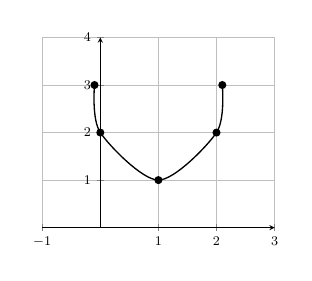
\begin{tikzpicture}[scale=0.6]
        \begin{axis}[
                grid = major,
                xmin=-1, xmax=3,
                ymin=0, ymax=4,
                axis lines=center,
                axis on top=true,
                small,
            ]
            \addplot[smooth, thick, color = black, mark = *]
            table[meta=label] {
                x       y       label
                -0.1    3       a
                0       2       a
                1       1       a
                2       2       a
                2.1     3

            };           
        \end{axis}
        \end{tikzpicture} 
        \caption{polynomial of degree 2}
    \end{subfigure}
\end{figure}


\parahead{In the PVSS protocol} we will use a simplified version of Lagrange interpolation formula. So instead of recovering the polynomium we just recover the evaluation in zero. The following will happen if take the formula \begin{math} \lambda_i(x)=\prod\limits_{j\in C,j\neq i}  \frac{x-j}{i-j} \end{math} and evaluate in zero \begin{math} \lambda_i(0)=\prod\limits_{j\in C,j\neq i}  \frac{0-j}{i-j} = \frac{j}{j-i} \end{math}. We reduce the formula by evaluating in $0$ and then one can multiply the numerator and denominator by $-1$ and then we get a the above formula.


\noindent
\begin{infobox}[Computing the coefficients for 3 tallier]
\begin{math}\lambda_1(0)=\prod\limits_{j\in C,j\neq 1} \frac{2}{2-1}  \cdot  \frac{3}{3-1} =\frac{3}{1} = 3 \end{math}\\
\begin{math}\lambda_2(0)=\prod\limits_{j\in C,j\neq 2} \frac{1}{1-2}  \cdot  \frac{3}{3-2} =\frac{1}{-1} \cdot  \frac{3}{1} =-1 \cdot  3=-3 \end{math}\\
\begin{math}\lambda_3(0)=\prod\limits_{j\in C,j\neq 3} \frac{1}{1-3}  \cdot  \frac{2}{2-3} =\frac{1}{-2} \cdot  \frac{2}{-1} =1 \end{math}\\
\textcolor{red}{Question to Ignacio: In our simpel example we have hardcoded and used these values but, if we want to compute the protocol with large values, can we still use these values or do we have to take other things into account?}
\label{info:Computing_the_coefficients}
\end{infobox}


\clearpage
\section{Electronic voting Protocol}
The PVSS protocol is a protocol which can handle a large set of secret data but it can also handle a small set data. This means that one of its applications is a  electronic voting system where the secret may differ from 0 or 1. The PVSS protocol differs from standard MPC protocol in which the shares are made public and verifiable.\\\\
This section will start by explaining our requirements for our implementation and after that we will explain the protocol. The main part will be the Ballot casting where the voter distribute their shares and the Tallying where the tallier computes and reconstructs the votes. The last part will go in depth with the mathematical proofs. \\

\noindent

\begin{infobox}[Short overview of the protocol]
\begin{enumerate}
\item Each voter signs it name on the bulletin board
\item Each tallier generates a private and a public key
\item Each tallier registries their public keys on the bulletin board
\item Initialization
\begin{enumerate}
\item The bulletin board generates and publish $g$ and $G$ and a securetity parameter $t$
\end{enumerate}
\item Ballot casting
\begin{enumerate}
\item Each voter votes $1$ or $0$
\item Each voter generates a random secret
\item Each voter creates shares of the secret to each tallier and encrypts it with the corresponding public key of the tallier. Each voter supply this secret share with evidence of its consistency with a $DLEQ$ proof
\item Each voter supply evidence for a valid vote with $PROOF_U$
\end{enumerate}
\item Tallying
\begin{enumerate}
\item At least $t-1$ tallier accumulates and decrypts their shares
\item One authority completes the final computation of the total votes
\end{enumerate}
\end{enumerate}
\end{infobox}

\noindent
In the following we will describe the central parts of the protocol. We will use terms as Tallying which in this context those who counts the votes.

\subsection{Initialization}



\parahead{Strong prime} In our implementation we will pick a prime, \begin{math}q\end{math}, so we avoid doing the gcd computation. The protocol states that we have to compute in a group of order q. This means that when we are doing operations in the exponent this property should be satisfied \begin{math}g^q=1\end{math} where \begin{math}q\end{math} is prime. If we are doing \begin{math}mod \ q \end{math} in the exponent we have \begin{math}g^q=g^0\end{math}. The reason for doing operation in the exponent \begin{math}mod \ q\end{math} is because we are using Sharmir secret sharing which require a finite field.\\\\
One can see that if \begin{math}q\end{math} is a prime say \begin{math}q=5\end{math}, then \begin{math}2^5 \ mod \ 5 = 32 \ mod \ 5 = 2\end{math}. For this to be true, we take the square of numbers modulo a prime in this form \begin{math}2q+1\end{math}. This is also called a strong prime. By using this mathematical structure this property holds. We can choose \begin{math}b=a^2\end{math}. Then we see the property holds \begin{math}b^{2q} = 1 \ mod \ 2q+1\end{math}. By example it is clear that \begin{math}(2^2)^5 \ mod \ 11 = 1024 \ mod \ 11 = 1\end{math}. Fermat little theorem states that \begin{math}b^{q-1} \ mod \ q = 1\end{math} where \begin{math}q\end{math} is prime. So we know if we pick our \begin{math}q\end{math} and \begin{math}b\end{math} (as a square)  in this form \begin{math}(b^{2})^{q+1-1} \ mod \ 2q+1 =1 =  b^{2q} \ mod \ 2q+1 =1\end{math} the property holds.

\noindent
\begin{infobox}[The bulleting board generates]
Public elements:\\
\begin{math}f \in_R \{1,...,2q\} \rightarrow g= f^2 \ mod\ 2q+1\end{math}\\
\begin{math}F \in_R \{1,...,2q\}\rightarrow G= F^2 \ mod\ 2q+1 \wedge G\neq1\end{math}\\
Security parameter:\\
\begin{math} t \in_R \Z_q^* = \{1,2,3,...,q-1\} \end{math}
\end{infobox}


\noindent
There are \textit{m} voters and \textit{n} talliers. For efficiency we will limit the computation of the votes to a finite number of talliers. 

\noindent
\begin{infobox}[The tallier generates a private and a public keys]
Private key: \begin{math}x_{i} \in_R \Z_q^* = \{1,2,3,...,q-1\}\end{math}\\
Public key: \begin{math}y_i=G^{x_i} ,\ i=\{1,2,3,...., n \}  \end{math}
\end{infobox}


\noindent
Every voter either votes "no" or "yes" corresponding to 0 or 1. The voter select a random secret value \begin{math}s \end{math}. The PVSS protocol is then used to distribute shares which contain a combination of the random secret and the vote. Every voter will construct a random polynomium at degree $t$ and then evaluate the shares  of each of the talliers.


\noindent
\begin{infobox}[The voter computes]
Vote: \begin{math}v\in\{0,1\} \end{math}\\
Random value: \begin{math} s\in_R \Z_q \end{math}\\ 
Shamir Secret Sharing: \begin{math} p(x)=s+\alpha_1x^1+\alpha_2x^2+,...,+\alpha_{t-1}x^{t-1}, \ \alpha_j\in_R \Z_q  \end{math}\\
Secret Shares: \begin{math} p(0)=s,\ p(1),\ p(2),...,\ p(n) \end{math}
\end{infobox}

\subsection{Ballot casting}
The  Ballot casting consists of \textit{distribution of the shares} and \textit{verification of the shares}. First the voter votes and then creates a random value. Two proofs are included by the voter a $DLEQ$ and a $PROOF_U$.\\

\noindent
\parahead{Shamir Secret Sharing} The \begin{math}p(i)\end{math} is the secret where we use Shamir Secret Sharing. The \begin{math}\alpha_j\end{math} is all the coefficients. The \begin{math}X_i\end{math} means the i'th tallier. \\

\noindent
\parahead{DLEQ} With DLEQ we prove that the exponent are equal \begin{math}X_i=g^{p(i)}  \land Y_i=y_i^{p(i)} \end{math} without revealing \begin{math}{p(i)} \end{math}. Note that there has been no communcation between the the player for now. We will present an interactive and a non-interactive proof of the DLEQ between the voter and the verifier.\\

\noindent
\parahead{\begin{math} PROOF_U \end{math}} With \begin{math} PROOF_U \end{math} the voter proofs "consistency" and that the vote is either 1 or 0.\\

\noindent
Note that the contruction of $Y_i$ is a hard problem to solve as we discussed in the discrete logarithm section. 

\begin{infobox}[Distribution of the shares by every voter]
The following gets publish to the bulleting board\\
\begin{math}Y_i=y_i^{p(i)} \end{math}, \begin{math}1\leq i\leq n\end{math} (Encryption of the share) \\ 
\begin{math}C_j=g^{\alpha_j},\ j=\{0,1,2,3,....,t-1 \} \end{math} \\ 
\begin{math}X_i=\prod\limits_{j=0}^{t-1} C_j^{i^j} =g^{p(i)}\end{math}, \begin{math}1\leq i\leq n\end{math}\\
\begin{math}U=G^{s+v} \end{math}\\
\begin{math}PROOF_U \end{math} and DLEQ
\end{infobox}



\parahead{Example} For clarification an example on \begin{math}X_i\end{math} calculations to tallier 1, tallier 2 and tallier 3.\\
Tallier 1: \begin{math}X_1=\prod\limits_{j=0}^{t-1} C_j^{i^j} = C_0^{1^0} * C_1^{1^1} * C_2^{1^2}\end{math}\\
Tallier 2: \begin{math}X_2=\prod\limits_{j=0}^{t-1} C_j^{i^j} = C_0^{2^0} * C_1^{2^1} * C_2^{2^2}\end{math}\\
Tallier 3: \begin{math}X_3=\prod\limits_{j=0}^{t-1} C_j^{i^j} = C_0^{3^0} * C_1^{3^1} * C_2^{3^2}\end{math}



\subsection{Tallying}
Tallying is the process of counting the votes. Here the tallier uses their private keys to collectively compute the final tally, based on the valid ballots.\\


\noindent
\parahead{Homomorphic secret sharing} property ensures that each tallier will  be able to multiply the shares and decrypt. Note that \textit{i} is referring to tallier 1, tallier  2 and tallier 3 and \textit{j} is referring to voter 1, voter 2 and voter 3.:\\

\begin{infobox}[The tallier decrypts the shares]
\begin{math}Y_i^*=(\prod\limits_{j=1}^{m} Y_{ij}) \ (mod\ 2*q+1) =y_i^{\sum\limits_{j=1}^m p_j(i)}\end{math}\\ \\
Following can be reduced by using the talliers private key. Note that we are raising to the multiplicative inverse of the private key in  \textit{q}:\\\\
\begin{math}y_i^{\sum\limits_{j=1}^m p_j(i)}=(G^{x_i})^{\sum\limits_{j=1}^m p_j(i)} = G^{x_i \sum\limits_{j=1}^m p_j(i)}= (G^{x_i \sum\limits_{j=1}^m p_j(i)})^{\frac{1}{x_i}}= G^{ \sum\limits_{j=1}^m p_j(i)}   \end{math}
\end{infobox}


\parahead{Example} on the multiplcation of the $Y_{ij}$\\
Voter 1: \begin{math}Y_{1,1}=y_{1,1}^{p_1(1)} \end{math}, \begin{math}Y_{2,1}=y_{2,1}^{p_2(2)} \end{math},.., \begin{math}Y_{n,1}=y_n^{p_n(n)} \end{math}\\
Voter 2: \begin{math}Y_{1,2}=y_{1,2}^{p_1(1)} \end{math}, \begin{math}Y_{2,2}=y_{2,2}^{p_2(2)} \end{math},.., \begin{math}Y_{n,2}=y_n^{p_n(n)} \end{math}\\
Voter \textit{m}: \begin{math}Y_{1,m}=y_{1,m}^{p_1(1)} \end{math}, \begin{math}Y_{2,m}=y_{2,m}^{p_2(2)} \end{math},.., \begin{math}Y_{n,m}=y_n^{p_n(n)} \end{math}\\

\noindent
Example on $Y_i^*$ is each tallier can publish the following. Note that every talliers exponent is the evaluation in some point in a given polynomium \begin{math}h(1), h(2),..., h(n) \end{math}.\\
Tallier 1 publish: \begin{math}Y_1^* = G^{ \sum\limits_{j=1}^m p_j(1)}   \end{math}\\
Tallier 2 publish: \begin{math}Y_2^* = G^{ \sum\limits_{j=1}^m p_j(2)}   \end{math}\\
Tallier \textit{n} publish: \begin{math}Y_n^* = G^{ \sum\limits_{j=1}^m p_j(n)}  \end{math}\\


\parahead{Lagrange interpolation} One can now use lambda, which is computed from the  Lagrange interpolation formular, \begin{math} \lambda_j \end{math} and multiply these values which will be the same as the sum of the exponents. See figure \ref{info:Computing_the_coefficients} \\

\noindent
The \begin{math}p_j(0) \end{math} correspond to the sum of the secret values of \textit{s} for the voters. This \begin{math}p_j(0)\end{math} corresponds to the evaluation of \begin{math}h(0)\end{math}. See figure  \ref{info:Applying_Lagrange_polynomial_interpolation}

\begin{infobox}[A master authority applies Lagrange interpolation]
\begin{math}(Y_1^*)^{\lambda_1 * \ (mod \ q)} * (Y_2^*)^{\lambda_2 \ (mod \ q)} * (Y_n^*)^{\lambda_n \ (mod \ q)} \ (mod \ 2*q+1) \end{math}\\


\noindent
We can substitute the $Y^*$ with $G$. The final result in the exponents is a evaluation in some polynomium in $0$ which corresponds to the sum of all random values $s$\\


\noindent
$=G^{ \sum\limits_{j=1}^m \lambda_j p_j(1)} \cdot G^{ \sum\limits_{j=1}^m \lambda_j p_j(2)} \cdot...\cdot G^{ \sum\limits_{j=1}^m \lambda_j p_j(n)} $\\
$=G^{ \sum\limits_{j=1}^m \lambda_j p_j(1) +  \sum\limits_{j=1}^m \lambda_j p_j(2) +...+  \sum\limits_{j=1}^m \lambda_j p_j(n)} $\\
$=G^{ \sum\limits_{j=1}^m (\lambda_j p_j(1)+\lambda_j p_j(2)+,...,+\lambda_{j}p_j(n))} = G^{ \sum\limits_{j=1}^m p_j(0)}= G^{ \sum\limits_{j=1}^m s_j}  $
\end{infobox}



\noindent
The last step is to isolate the votes and then compute the final result.


\noindent
\begin{infobox}[A master authority computes the votes]
By combining \begin{math}U_j \end{math} we obtain: \\ 
\begin{math} (\prod\limits_{j=1}^{m} U_{j}) \ (mod \ 2*q+1)=  G^{ \sum\limits_{j=1}^m s_j +v_j}\end{math} \\ \\
By dividing we isolate \textit{v}: \\ \\
\begin{math}\frac{G^{ \sum\limits_{j=1}^m s_j +v_j}}{{ G^{ \sum\limits_{j=1}^m s_j} }} =G^{ \sum\limits_{j=1}^m s_j +v_j -\sum\limits_{j=1}^m s_j} = G^{ \sum\limits_{j=1}^m v_j}  \end{math}
\end{infobox}


\parahead{Exhaustive search} To solve the computing of the votes one can compute \begin{math}G^0, G^1, G^3,..., G^{v_j} \end{math} by exhaustive search. 

\parahead{Baby-step giant-step} A more efficient algorithm is to use Baby-step giant-step algorithm. 


%************Proofs start
\subsection{Proofs}
In this section we will elaborate the mathematical justification of the interactive- and non interactive DLEQ and the $PROOF_U$. 
%----------------------------------------------------------------------
\subsubsection{DLEQ interactive proof between voters and verifier}
%----------------------------------------------------------------------
DLEQ stands for discrete logarithm equality and it proofs the exponent are equal \begin{math}X_i=g^{p(i)}  \land Y_i=y_i^{p(i)} \end{math} without revealing \begin{math}{p(i)} \end{math}. The verification of the shares in the interactive proof happens by the following  interaction between the prover and the verifier.\\\\

\noindent
\parahead{The prover computes}  \begin{math}a_1=g^w  \land a_2=y_i^w,  w\in_R \Z_q \end{math} and sends $a_1$ and $a_2$ to the verifier. \parahead{ The verifer computes}  \begin{math}C\in_R \Z_q \end{math} and sends $C$ to the prover. \parahead{The prover computes}  \begin{math}r=w-p(i) * C\end{math}. \parahead{ The verifer computes}  if the following computation is true \begin{math}a_1 = g^r*X_i^C \ \land \ a_2=y_i^r*Y_i^C\end{math}.


\begin{figure}[H]
    \centering        
    
    $
    \begin{array}{l}
    \hline                      \
    \textbf{DLEQ protocol}      \\
    \hline                      \
    Public:  g,X_i,y_i,Y_i       \\
    \\
	\begin{array}{L{2cm}ccc}
        & \text{\textsf{Prover}} & & \text{\textsf{Verifier}} \\
        \hline
        Step \ 1 & w\in_R \Z_q & & \\
        & a_1=g^w     & & \\
        & a_2=y_i^w   & \xrightarrow{\hspace{1em}a_1 \land a_2\hspace{1em}} & \\
        Step \ 2 & & & C\in_R \Z_q \\
        & & \xleftarrow{\hspace{2em}C\hspace{2em}} & \\
        Step \ 3 & r=w-p(i) * C    & & \\
        Step \ 4 & & \xrightarrow{\hspace{2em}r\hspace{2em}} & \begin{array}{c}
        checks \ if: \\      
        a_1 = g^r*X_i^C \\ 
        a_2=y_i^r*Y_i^C
        \end{array} \\
        \hline
    \end{array}
    \end{array}
    $    
    \caption{DLEQ interactive}
	\label{fig:DLEQ}
\end{figure}
	


\noindent
Note that the verifier sends a challenge \textit{C}, after the prover has computed \begin{math}a_1\end{math} and  \begin{math}a_2\end{math}. The check only passes if the prover used the same exponents. The proof shows that there exist some element \begin{math} \alpha\end{math} such that \begin{math}g^\alpha = X_i \ \land \ y_i^\alpha=Y_i \end{math} where  \begin{math} \alpha\end{math} is equal to  \begin{math} p(i)\end{math}. The following is an argument why DLEQ works.\\ 

\noindent
\parahead{Example} We will now show a concrete example why the challenge matters. Say that the challenge doesnt matter it will be the same as saying that the challenge is 1. 

\begin{infobox}[DLEQ without a challenge]
Prover \begin{math}\rightarrow\end{math} Verifier: \begin{math}a_1=g^6 \ \land\ a_2=y_i^7 \ \land \ X_i=g^2 \ \land \ Y_i=y_i^3 \end{math}\\
Verifier \begin{math}\rightarrow\end{math} Prover: \begin{math}C=1 \end{math}\\
Prover \begin{math}\rightarrow\end{math} Verifier: \begin{math}r=w-p(i) * C = 6-2 * 1= 4\end{math}\\
Verifier knows:  \begin{math}a_1=g^4 * X_i \ \land \ a_2=y_i^4 * Y_i \end{math}\\
Verifier checks if:  \begin{math}a_1 = g^4*X_i^C = g^4*g^{2*1} = g^6\end{math}\\
Verifier checks if:  \begin{math} a_2=y_i^4 * Y_i^C = y_i^4 * y_i^{3*1}= y_i^7 \end{math}
\end{infobox}

\noindent
One can see that both checks passes in this example despite that the prover is dishonest. Next example shows the verification with a challenge.

\begin{infobox}[DLEQ with a challenge]
Prover \begin{math}\rightarrow\end{math} Verifier: \begin{math}a_1=g^6 \ \land\ a_2=y_i^7 \ \land \ X_i=g^2 \ \land \ Y_i=y_i^3 \end{math}\\
Verifier \begin{math}\rightarrow\end{math} Prover: \begin{math}C=9\ (mod \ 5) \end{math}\\
Prover \begin{math}\rightarrow\end{math} Verifier: \begin{math}r=w-p(i) * C = 6-2 * 4 \ (mod \ 5)= 3\end{math}\\
Verifier knows:  \begin{math}a_1=g^3 * X_i \ \land \ a_2=y_i^3 * Y_i \end{math}\\
Verifier checks if:  \begin{math}a_1 = g^3*X_i^C = g^3*g^{2*4} = g^3 * g^3 = g^6= g^1= g\end{math}\\
Verifier checks if:  \begin{math} a_2=y_i^3 * Y_i^C = y_i^3 * y_i^{3*4}= y_i^3 * y_i^{1*2}= y_i^3 * y_i^2= y^5=y^0= 1 \end{math}
\end{infobox}


\parahead{The mathematical justification} Verifier knows that the prover has raised \begin{math}g^w\end{math} and \begin{math}y_i^w\end{math}. We denote these exponents by \begin{math}w\end{math}    and \begin{math}w^{'}\end{math}. The verifier also knows that the prover has computed \begin{math}X_i=g^{p(i)}  \land Y_i=y_i^{p(i)} \end{math}. We denote the exponents by \begin{math}m_i\end{math} and \begin{math}m_i^{'}\end{math}. We know
\begin{math} a_1= g^w \end{math} equal to \begin{math}g^r * X_i^C=g^r*g^{m_i*C} = g^{r+m_i*C}\end{math} and
\begin{math} a_2= y_i^{w^{'}}\end{math} equal to \begin{math}y_i^r * Y_i^C=y_i^r*y_i^{m_i^{'}*C} = y_i^{r+m_i^{'}*C}\end{math}.
Based on this we can now write two inequalities. It is unlikely that if the prover was dishonest that these two checks passes. It may not be clear but in order for these inequalities to be true we can rewrite.

\begin{infobox}[DLEQ mathematical justification]
We know\\
\begin{math} a_1= g^w \end{math} equal to \begin{math}g^r * X_i^C=g^r*g^{m_i*C} = g^{r+m_i*C}\end{math}\\
\begin{math} a_2= y_i^{w^{'}}\end{math} equal to \begin{math}y_i^r * Y_i^C=y_i^r*y_i^{m_i^{'}*C} = y_i^{r+m_i^{'}*C}\end{math}\\\\
We can now write two inequalities\\
\begin{math} w= r+m_i * C\ (mod\ q) \implies r= w-m_i*C\ (mod\ q) \end{math}\\
\begin{math} w^{'}= r+m_i^{'} * C\ (mod\ q) \implies r= w^{'}-m_i^{'} * C\ (mod\ q) \end{math}\\\\
These two inequalities has to be equal, therefor we can rewrite\\
\begin{math}w-m_i*C = w^i-m_i^{'}\ (mod\ q) \implies (w-w^i)-(m_i - m_i^{'}) * C = 0 \ (mod\ q) \end{math}
\end{infobox}


\noindent
The prover has to be honest if this equation must be true. It is very unlikely that, if the prover has been dishonest that he will succeed. Since the prover doesn't know the challenge the probability will be \begin{math} \frac{1}{q}\end{math}.


\begin{infobox}[Zero knowledge proof for the DLEQ]
\textcolor{red}{Question to Ignacio: we need to have clear separation on what is referring to what in our description of the proof}\\\\
\parahead{Completeness:} If the prover is honest it should pass or if the statement is true, the honest verifier (that is, one following the protocol properly)
will be convinced of this fact by an honest prover.\\\\
\parahead{Soundness:}If the statement is false then it should fail with large probability or if the statement is false, no cheating prover can convince
the honest verifier that it is true, except with some small probability?\\\\
\parahead{Zero-knowledge:} If the statement is true, no cheating verifier learns anything other than the fact that the statement is true.?
\end{infobox}

%----------------------------------------------------------------------
\subsubsection{DLEQ non-interactive proof between voters and verifier}
%----------------------------------------------------------------------
Here we present how one can turn an interactive proof to a non interactive proof.

\parahead{Fiat Shamir} This is also known as the Fiat Shamir where we are transforming a interactive proof into a non interactive proof (signature scheme). Instead of the verifier computes a challenge, the prover computes the challenge as a random function (hash).\\
\textcolor{red}{We will describe an non optimized and a optimized version - does this have a name??}\\


\parahead{The prover computes} \begin{math}a_1=g^w \ (mod\ q)  \land a_2=y_i^w \ (mod\ q),  w\in_R \Z_q \end{math}. Then the prover computes the hash \begin{math}C=H(X_i,Y_i,a_1,a_2) \end{math}. Then the prover computes  \begin{math}r=w-p(i) * C \ (mod\ q)\end{math}. Last the prover publish \begin{math}a_1, a_2,r,C\end{math}. \\

\noindent
\parahead{The verifier computes} the following computations \begin{math}a_1 = g^r*X_i^C  \ (mod\ q)\end{math} and \begin{math} a_2=y_i^r * Y_i^C \ (mod\ q)\end{math} and \begin{math}C=H(X_i,Y_i,a_1,a_2)\end{math}.


\begin{figure}[H]
    \centering        
    
    $
    \begin{array}{l}
    \hline                      \
    \textbf{DLEQ protocol}      \\
    \hline                      \
    Public:  g,X_i,y_i,Y_i       \\
    \\
	\begin{array}{L{1.1cm}lcl}
        & \text{\textsf{Prover}} & & \text{\textsf{Verifier}} \\
        \hline
        Step \ 1    &           \begin{array}{l}
                                    w\in_R \Z_q             \\ 
                                    a_1=g^w \ (mod\ q)      \\ 
                                    a_2=y_i^w \ (mod\ q)    \\
                                    C=H(X_i,Y_i,a_1,a_2)    \\
                                    r=w-p(i) * C \ (mod\ q)
                                \end{array}     &               & \\
                    &                   &               & \\
        Step \ 2    &                   &               \xrightarrow{\hspace{0.4em}a_1 , a_2 , r , C\hspace{0.4em}} & \begin{array}{l}
            checks \ if: \\      
            a_1 = g^r*X_i^C \\ 
            a_2=y_i^r*Y_i^C \\
            C=H(Xi,Yi,a1,a2)
        \end{array} \\
        \hline
    \end{array}
    \end{array}
    $    
    \caption{DLEQ non interactive}
	\label{fig:DLEQ_1}
\end{figure}


\noindent
 Note in above that there is no interaction between the prover and the verifier. In the following we will show how one can improve the amount of computation of the challenge \textit{C}. Instead of computing the challenge \textit{n} times, one can compute it once and reuse the challenge.





\begin{infobox}[DLEQ optimized]
DLEQ \begin{math}(g,X_i,y_i,Y_i) \end{math} for  \begin{math}1\leq i \leq n \end{math}  \\
Prover publish: \begin{math}a_{1,i}=g^{w_i} \ (mod\ q)  \land a_{2,i}=y_i^{w_i} \ (mod\ q),  w_i\in_R \Z_q \end{math}\\
Prover computes the hash: \begin{math}C=H(X_i,Y_i,...,X_n,Y_n,a_{1,1},a_{2,1},\\a_{1,2},a_{2,2},...,a_{1,n},a_{2,n})\end{math}\\
Prover computes \begin{math}r_i\end{math}:  \begin{math}r_i=w_i-p(i) * C \ (mod\ q)\end{math}\\
Prover publish:  \begin{math}r_i,C\end{math}\\
Verifier checks if:  \begin{math}a_{1,i} = g^{r,i}*X_i^C \ (mod\ q) \end{math}\\
Verifier checks if:  \begin{math} a_{2,i}=y_i^{r_{i}} * Y_i^C \ (mod\ q)\end{math}\\ 
Verifier checks if:  \begin{math}C=H(X_i,Y_i,...,X_n,Y_n,a_{1,1},a_{2,1},a_{1,2},a_{2,2},...,a_{1,n},a_{2,n})\end{math}

\label{info:DLEQ_optimized}
\end{infobox}

\parahead{Example} Hence the hash contains all the  \begin{math}a_i \end{math} the prover will compute this proof once for all  \begin{math}p(i) \end{math} which improve efficiency. This means that if there are 3 voters, then the above computation has to be done 3 times for every tallier, but same hash can be computed once for every tallier. 

\begin{infobox}[DLEQ computation for 3 voters]
Prover publish:  $a_{1,1},a_{2,1},a_{1,2},a_{2,2},a_{1,3},a_{2,3}$ \\
Prover publish:                   $C,r_1,r_2,r_3$ \\
Prover selects:  $w_1, w_2,w_3\in_R \Z_q$ \\
Prover computes: $a_{1,i}=g^w_i \ (mod\ q) \land a_{2,i}=y_i^{w_i} \ (mod\ q)$ \\
Prover computes the hash:  $C=H(X_i,Y_i,...,X_n,Y_n,a_{1,1},a_{2,1},$\\
$a_{1,2},a_{2,2},...,a_{1,n},a_{2,n})$\\
Prover computes  $\ r_i:  r_i=w_i-p(i) * C \ (mod\ q)$ \\\\
The verification contains the following computation: \\
Verifier checks if: $a_{1,i} = g^{r,i}*X_i^C \ (mod\ q) $        \\
Verifier checks if: $a_{2,i} =y_i^{r_{i}} * Y_i^C \ (mod\ q)  $   \\
Verifier checks if: $C=H(X_i,Y_i,...,X_n,Y_n,a_{1,1},a_{2,1},a_{1,2},a_{2,2},...,a_{1,n},a_{2,n})$

\end{infobox}



\begin{infobox}[Zero knowledge proof for the DLEQ]
\textcolor{red}{Question to Ignacio: we need to have clear separation on what is referring to what in our description of the proof}\\\\
\parahead{Completeness:} If the prover is honest it should pass or if the statement is true, the honest verifier (that is, one following the protocol properly)
will be convinced of this fact by an honest prover.\\\\
\parahead{Soundness:}If the statement is false then it should fail with large probability or if the statement is false, no cheating prover can convince
the honest verifier that it is true, except with some small probability?\\\\
\parahead{Zero-knowledge:} If the statement is true, no cheating verifier learns anything other than the fact that the statement is true.?
\end{infobox}

%----------------------------------------------------------------------
\subsubsection{Description of $ \mathbf{PROOF_U} $}
%----------------------------------------------------------------------
In this section we will show the interactive proof. Through Fiat–Shamir  we transform an interactive proof of knowledge into a non-interactive proof of knowledge. First of all the voter proves that there is consistency between the exponents of how \begin{math}U\end{math} and \begin{math}C_0\end{math} is constructed from \begin{math}U=G^{s+v}\end{math} and \begin{math}C_0 = g^s\end{math}. The exponents only differs from the vote hence 0 or 1.\\

\begin{figure}[H]
    \centering        
    
    $
    \begin{array}{l}
    \hline                      \
    \textbf{$PROOF_U$ protocol}      \\
    \hline                      \
    Public:  U=G^{s+v},\ C_0=g^s       \\
    \\
	\begin{array}{L{1.4cm}lcr}
        & \text{\textsf{Prover}} & \text{\textsf{Verifier}} \\
        \hline
        Step \ 1a   &           \begin{array}{l}
                                    v=0             \\ 
                                    w\in_R \{1,...,q-1\}, \\ 
                                    r_1\in_R\{1,...,q-1\},\\
                                    d_1\in_R\{1,...,q-1\},      \\ 
                                    a_0 = g^w,\\ 
                                    a_1 = g^{r_1}*C^{d_1}_0,\\ 
                                    b_0 = G^w,  \\
                                    b_1 = G^{r_1} * (\frac{U}{G^{1-v}})^{d_1} = G^{r_1} * (\frac{U}{G})^{d_1} \\
                                \end{array}     &               & \\
                                \\
                    &                   \xrightarrow{\hspace{1em}a_0, a_1, b_0, b_1\hspace{1em}} \ \textbf{Publish to bulletin}&  & \\                                
                    &                   &               & \\
        Step \ 1b   &           \begin{array}{l}
                                    v=1             \\ 
                                    w\in_R \{1,...,q-1\},\\ r_0\in_R\{1,...,q-1\},\\
                                    d_0\in_R\{1,...,q-1\},      \\ 
                                    a_0 = g^{r_0}*C^{d_0}_0,\\
                                    a_1 = g^w,\\
                                    b_0 = G^{r_0} * (\frac{U}{G^{1-v}})^{d_0}= G^{r_0} * U^{d_0} ,\\
                                    b_1 = G^w\\
                                \end{array}     &               & \\
                    &                   &               & \\
                    \\
                    &                   \xrightarrow{\hspace{1em}a_0, a_1, b_0, b_1\hspace{1em}} \ \textbf{Publish to bulletin} & \\
        Step \ 2    &                    & \begin{array}{l}
                                \textbf{Create \ challenge:} \\      
                                C\in_R \{0,...,q-1\} \\ 
                                \xleftarrow{\hspace{2em}C\hspace{2em}}\\
                                \end{array}  \\
        Step \ 3a   &          \begin{array}{l}
                                   v=0             \\ 
                                   d_0= C-d_1\ mod\ q,\\
                                   r_0=w-s*d_0 \ mod\ q\\  
                                \end{array}     &               & \\
                                \\
                    &                   \xrightarrow{\hspace{1em}d_0,\ r_0,\ d_1,\ r_1\hspace{1em}} \ \textbf{Publish to bulletin}&  & \\                                
                    &                   &               & \\
        Step \ 3b   &           \begin{array}{l}
                                    v=1             \\ 
                                    d_1= C-d_0\ mod\ q, \\
                                    r_1=w-s*d_1 \ mod\ q\\ 
                                \end{array}     &               & \\
                                \\
                    &                   \xrightarrow{\hspace{1em}d_0,\ r_0,\ d_1,\ r_1\hspace{1em}} \ \textbf{Publish to bulletin}&  &\\
                    &                   &               & \\
        Step \ 4   &                    & \begin{array}{l}
                                \textbf{Verification:} \\      
                                C = d_1 + d_0,\\
                                a_0=g^{r_0} * C^{d_1}_0,\\
                                b_0 = G^{r_0}*U^{d_0},\\
                                a_1=g^{r_1} * C^{d_1}_0,\\
                                b_1= G^{r_1} *(\frac{U}{G})^{d_1} \\ 
        \end{array} \\
        \hline
    \end{array}
    \end{array}
    $    
    \caption{$PROOF_U$}
	\label{fig:DLEQ}
\end{figure}

\parahead{Explanation of the protocol} In step 1 the voter publish \begin{math}a_0,\ b_0,\ a_1,\ b_1\end{math}. Note that the difference between voting 0 or 1 is just by swapping the values between the variables \begin{math}a_0,\ b_0\end{math} and \begin{math}a_1,\ b_1\end{math}. The point is that the verifier will not be able to distinguish the value of the vote and thereby gain knowledge about the vote.

\noindent
\begin{infobox}[Step 1]
Voter votes 0 and creates and publish:\\
\begin{math}v=0,\ w\in_R \{1,...,q-1\},\ r_1\in_R\{1,...,q-1\},\ d_1\in_R\{1,...,q-1\}\end{math}\\
Publish: \begin{math}a_0 = g^w,\ b_0 = G^w,\ a_1 = g^{r_1}*C^{d_1}_0,\ b_1 = G^{r_1} * (\frac{U}{G^{1-v}})^{d_1} = G^{r_1} * (\frac{U}{G})^{d_1} \end{math}\\\\
Voter votes 1 and creates and publish\\
\begin{math}v=1,\ w\in_R \{1,...,q-1\},\ r_0\in_R\{1,...,q-1\},\ d_0\in_R\{1,...,q-1\}\end{math}\\
Publish: \begin{math}a_1 = g^w,\ b_1 = G^w,\ a_0 = g^{r_0}*C^{d_0}_0,\ b_0 = G^{r_0} * (\frac{U}{G^{1-v}})^{d_0}=  G^{r_0} * U^{d_0} \end{math}
\end{infobox}

\noindent
\begin{infobox}[Step 2]
The verifier creates a challenge \begin{math}C\in_R \{0,...,q-1\}\end{math} to the voter.
\end{infobox}

\noindent
The outcome from step 3 is that the voter publish \begin{math}d_0,\ r_0,\ d_1,\ r_1\end{math}. Note that the voters computation depends on the challenge from the interaction between the verifier.

\noindent
\begin{infobox}[Step 3]
Voter votes 0 computes\\
\begin{math}v=0,\ d_0= C-d_1\ mod\ q, \ r_0=w-s*d_0 \ mod\ q\end{math}\\\\
Voter votes 1 computes\\
\begin{math}v=1,\ d_1= C-d_0\ mod\ q, \ r_1=w-s*d_1 \ mod\ q\end{math}
\end{infobox}

\noindent
In step 4 the verifier will be able computes and verify consistency.

\noindent
\begin{infobox}[Step 4]
\begin{math}C = d_1 + d_0,\ a_0=g^{r_0} * C^{d_1}_0,\ b_0 = G^{r_0}*U^{d_0},\ a_1=g^{r_1} * C^{d_1}_0,\ b_1= G^{r_1} *(\frac{U}{G})^{d_1}\end{math}
\end{infobox}

\parahead{Non-interactive proof} We can turn this into a non-interactive proof by replacing step 2 with the voter using a hash function and thereby avoiding interaction with the verifier. The prover will then compute a hash of \begin{math}C=H(U,\ C_0,\ a_0,\ b_0,\ a_1,\ b_1) \end{math}.\\\\

\parahead{Mathematical justification} The mathematical justification in step 4, we will replace with earlier expression from above and replace by the actual value of the vote.

\begin{infobox}[Explanation of \begin{math}a_0=g^{r_0} * C^{d_1}_0\end{math}]
vote=0, show that \begin{math}a_0=g^{r_0} * C^{d_0}_0 = g^w \end{math} is well constructed\\
\begin{math}a_0=g^{r_0} * C^{d_0}_0 = g^{w-sd_0}* g^{sd_0}= g^{w-sd_0+ sd_0}= g^w\end{math}\\
vote =1, this is trivial because \begin{math}a_0 \end{math}  is constructed from \begin{math}a_0=g^{r_0} * C^{d_0}_0 \end{math}
\end{infobox}


\begin{infobox}[Explanation of \begin{math}b_0 = G^{r_0}*U^{d_0}\end{math}]
vote=0, show that \begin{math}b_0 = G^{r_0}*U^{d_0} = G^w \end{math} is well constructed\\
\begin{math}b_0 = G^{r_0}*U^{d_0} =  G^{w-sd_0}*G^{(s+0)*d_{0}} =  G^{w-sd_0}*G^{sd_{0}}= G^w \end{math}\\
vote 1, show that \begin{math}b_0 = G^{r_0}*(\frac{U}{G^{1-1}})^{d_0}=  G^{r_0}*U^{d_0} \end{math} \\
\begin{math}b_0 = G^{r_0}*(\frac{U}{G^{1-v}})^{d_0}=  G^{r_0}*(\frac{U}{G^{0}})^{d_0} = G^{r_0}*(\frac{U}{1})^{d_0}=  G^{r_0}*U^{d_0}  \end{math}
\end{infobox}



\begin{infobox}[Explanation of \begin{math}a_1=g^{r_1} * C^{d_1}_0\end{math}]
vote= 1, show that \begin{math}a_1=g^{r_1} * C^{d_1}_0 = g^w \end{math} is well constructed\\
\begin{math}a_1=g^{r_1} * C^{d_1}_0 = g^{w-sd_1}* g^{sd_1}= g^{w-sd_1+ sd_1}= g^w\end{math}\\
vote =0, this is trivial because \begin{math}a_1 \end{math} is constructed from \begin{math}a_1=g^{r_1} * C^{d_1}_0 \end{math}
\end{infobox}


\begin{infobox}[Explanation of \begin{math}b_1= G^{r_1} *(\frac{U}{G})^{d_1}\end{math}]
vote=1, show that \begin{math}b_1= G^{r_1} *(\frac{U}{G})^{d_1} = G^W\end{math} is well constructed \\
\begin{math}b_1= G^{r_1} *(\frac{U}{G})^{d_1} = G^{w-sd_1}*(U*G^{-1})^{d_1}= G^{w-sd_1}* (G^{s+1})^{d_0}*G^{-d_1} =  G^{w-sd_1}* G^{sd_0+d_0}*G^{-d_1}= G^W\end{math}\\
vote=0, show that  \begin{math}b_1= G^{r_1} *(\frac{U}{G^{1-v}})^{d_1} = G^{r_1} *(\frac{U}{G})^{d_1}\end{math} is well constructed\\
\begin{math}b_1= G^{r_1} *(\frac{U}{G^{1-v}})^{d_1} = G^{r_1} *(\frac{U}{G^{1-0}})^{d_1} = G^{r_1} *(\frac{U}{G})^{d_1}\end{math}
\end{infobox}



\begin{infobox}[Zero knowledge proof for the $PROOF_U$]
\textcolor{red}{Question to Ignacio: we need to have clear separation on what is referring to what in our description of the proof}\\\\
\parahead{Completeness:} If the prover is honest it should pass or if the statement is true, the honest verifier (that is, one following the protocol properly)
will be convinced of this fact by an honest prover.\\\\
\parahead{Soundness:}If the statement is false then it should fail with large probability or if the statement is false, no cheating prover can convince
the honest verifier that it is true, except with some small probability?\\\\
\parahead{Zero-knowledge:} If the statement is true, no cheating verifier learns anything other than the fact that the statement is true.?
\end{infobox}

%----------------------------------------------------------------------
\subsubsection{DLEQ proof by the servers}
%----------------------------------------------------------------------
The tallier will do computations on each of their shares. Here each tallier uses the DLEQ to prove that the decryption of their shares is done correctly. We will first show the interactive proof and then transform it to a non-interactive proof. The input values are \begin{math}(G,\ y_i,\ S_i, Y_i)\end{math} where \begin{math}G = y_i^{x_i}\end{math} and  \begin{math} Y_i=S_i^{x_i}\end{math}. We have some initial values
 \begin{math}g_1 =G,\ h_i=y_i,\ g_2=S_i,\ h_2=Y_i,\ \alpha=x_i \end{math} and \begin{math}w \in_R \{0,...,q-1\}\end{math}.\\
 
 
 
\noindent 
In step 1 the prover computes \begin{math}a_1,\ a_2=S_i^w\end{math}. In step 2
the verifier creates a challenge \begin{math}C\end{math}. In step 3 the tallier computes \begin{math}r=w-C*x_i\end{math}. In step 4 the verifier computes \begin{math}a_1=G^r*y_i^C,\ a_2=S_i^r*Y_i^C\end{math}.
 
 
 
\begin{figure}[H]
    \centering        
    
    $
    \begin{array}{l}
    \hline                      \
    \textbf{DLEQ protocol}      \\
    \hline                      \
    Input:  G,\ y_i,\ S_i, \ Y_i \ where \ G = y_i^{x_i} \land Y_i=S_i^{x_i}     \\
    Output: 0 \ or \ 1
    \\
	\begin{array}{L{2cm}ccc}
        & \text{\textsf{Prover}} & & \text{\textsf{Verifier}} \\
        \hline
        Step \ 1 & w\in_R \Z_q & & \\
        & a_1=g^w     & & \\
        & a_2=y_i^w   & \xrightarrow{\hspace{1em}a_1 \land a_2\hspace{1em}} & \\
        Step \ 2 & & & C\in_R \Z_q \\
        & & \xleftarrow{\hspace{2em}C\hspace{2em}} & \\
        Step \ 3 & r=w-p(i) * C    & & \\
        Step \ 4 & & \xrightarrow{\hspace{2em}r\hspace{2em}} & \begin{array}{c}
        checks \ if: \\      
        a_1 = g^r*X_i^C \\ 
        a_2=y_i^r*Y_i^C
        \end{array} \\
        \hline
    \end{array}
    \end{array}
    $    
    \caption{DLEQ}
	\label{fig:DLEQ}
\end{figure} 
 
\parahead{Non-interactive proof} Note the interaction in step 2 where the verifier create a challenge to the server. Through Fiat–Shamir we transform an interactive proof of knowledge into a non-interactive proof of knowledge. We replace step 2 with a hashing algorithm  \begin{math}C=H(G,\ y_i,\ S_i,\ Y_i,\ a_1,\ a_2)\end{math}.\\
 
\parahead{Mathematical justification} For the mathematical justification in step 4, we can do the following computation on \begin{math}a_1=G^w\end{math} and \begin{math}a_2=S_i^w\end{math}.\\\\
Let \begin{math}a_1=G^w\end{math} we show that \begin{math}G^r*y_i^C=G^r*y_{x_i}^C=G^{r+x_iC}=G^{w-Cx_i+x_iC}=G^w\end{math}\\\\
Let \begin{math}a_2=S_i^w\end{math} we show that
\begin{math}S_i^r*Y_i^C=S^r*Y_{x_i^C}=S^{w-Cx_i}*S_i^{x_i*C}=S^{w-Cx_i+x_i*C}=S_i^w\end{math}



\begin{infobox}[Zero knowledge proof for the $DLEQ$ for the tallier]
\textcolor{red}{Question to Ignacio: we need to have clear separation on what is referring to what in our description of the proof}\\\\
\parahead{Completeness:} If the prover is honest it should pass or if the statement is true, the honest verifier (that is, one following the protocol properly)
will be convinced of this fact by an honest prover.\\\\
\parahead{Soundness:}If the statement is false then it should fail with large probability or if the statement is false, no cheating prover can convince
the honest verifier that it is true, except with some small probability?\\\\
\parahead{Zero-knowledge:} If the statement is true, no cheating verifier learns anything other than the fact that the statement is true.?
\end{infobox}
%************************* Proof end

\clearpage
\section{Security}
Passive corruption is that a player (semihonest) gets access to information which the player is not entitled to, e.g. if a player ask another player about his information and tries to compare the information and get some more information in that way. Active corruption happens when the players (malicious) try to send values that they are not supposed to send - so the players deviate from the protocol. By using secret sharing we can prevent passive corruption, because the scheme guaranties that if t-players are corrupted then they will not be able to gain anything. The scheme can be made secure against active cheating, but we will not look at the details of this case in this project.
We will look at the auction scheme where the farmers are not supposed to know other bids than their own. Therefor we will be concentrating on the passive corruption. 
When we are referring to an adversary, we mean a Monolithic Adversary who corrupts a set of players. This is the strongest form of corruption. Let us say we have 10 players and two adversaries. The first adversary corrupts one of the players and the other corrupts 2 players. Imagine if there was one adversary who corrupts three players. Then it would be the case that this adversary would have access to more information than the first situation with 2 adversaries.
\section{Simple voter application}

\begin{center}
\begin{algorithm}[H]
\KwIn{a set $V$ of $q$ queries $(v_i, c_i) \in \{0,1\}^{k+1}$ from the LPN Oracle, values $a, b$ such that $k = ab$}
\KwOut{values $\svec_1,...\svec_b$}
\SetKw{KwAnd}{and}
\SetKw{KwOr}{or}
\Begin{
Partitions the positions $a$ into disjoint $q_1 \cup...\cup q_{a-1}$ with $q_i$ of size $b$\;
\For{$i=1$ to $a-1$}{
  Partition $V = V_1 \cup ... \cup V_{2^b}$ s.t.vectors in $V_j$ have the same bit values on $q_i$\;
  \For{\textbf{each} $V_j$}{
    Choose a random $(v^*,c^*) \in V_j$ as a representative vector\;
    Replace each $(v,c)$ by $(v,c) \oplus (v^*,c^*), (v,c) \in V_j$ for $(v,c) \neq (v^*,c^*)$\;
    Discard $(v^*,c^*)$ from $V_j$\;
  }
  $V = V_1 \cup ... \cup V_{2^b}$\; 
  }
$f(x)=\sum_{i} 1_{v'_i}=x(-1)^{c'_i}$\;
$f(v)=\sum_{x} (-1)^{\dotp{v}{x}}f(x)$\;
$(\svec_1,...,\svec_b) = arg max(f(v))$
\Return{$\svec_1,...,\svec_b$}
}
\caption{LF1 Algoritmen som beskreven i [3]}
\end{algorithm}
\end{center}



\noindent
Quatilty attribute\\
Quatilty attribute drivers\\
QAW og Quality attribute scenario : skalerbarhed og sikkerhed\\
Tactics\\
3+1 viewpoints\\
Distributed patterns\\
Microservices: distributed randomness\\
Sikkerhed på en browser\\
Toplogi: stjerner ingen snakker med hinanden\\
Beslutning omkring valg af kodeplatform... er det arktikturmæssig beslutning... Måske decisional krutchen ??\\\\

\noindent
klient (voter)\\
tallier\\
oberserver (master authority)\\
bullutin board (server)\\
\noindent
Initielt\\
En klient melder sig til bullutin board. Får tildelt public værdier. \\
En tallier melder sig til bullutin board. \\\\
\noindent
Ballotcasting -> Nu starter voting ->  $DLEQ$ og $PROOF_U$ -> indenfor deadline\\
Tallying -> Optællingsfasen for hver \\
Master authority -> Endelig summering -> brute force -> publish samlet stemme -> en vote som ikke er valideret tæller ikke med -> logning af beregning \\\\

\noindent
Issue tables\\
Diskussion/ta stilling \\
Remote randomness / webbrowser / .NET\\
https\\
man må ikke dobbelt vote\\
store tal\\
hardware krav

\clearpage
\section{Bibliography}

\begin{thebibliography}{9}

\bibitem{levfou05}
  Eric Levieil and Pierre-Alain Fouque,
  \emph{An improved LPN algorithm},
  Paris Cedex 05, France, 2005.
  
\bibitem{BKW03}
  A. Blum, A. Kalai and H. Wasserman.
  \emph{Noise-tolerant Learning, the Parity Problem, and the statistical Query Problem},
  Journal of the ACM 50,4, July 2003, pp. 506-519.
  
\bibitem{BOTRVA}
  Sonia Bogos, Florian Tramér, and Serge Vaudenay
  \emph{On Solving LPN using BKW and Variants},
  {IACR} Cryptology ePrint Archive, 2015.  
  

\end{thebibliography}
\end{document}
